\chapter{Supernova neutrino bursts and physics with low-energy neutrinos}
\label{ch:snb-lowe}


%%%%%%%%%%%%%%%%%%%%%%%%%%%%%%%%%%%%%%%%%%%%%%%%%%%%%%%%%%%%%%
\section{Supernova neutrino bursts}
\label{sec:snb-lowe-snb}

The neutrinos from a core-collapse supernova are emitted in a burst of
a few tens of seconds duration, with about half the signal emitted in the first
second. The neutrino energies are mostly in the range \numrange{5}{50}{MeV}, and the 
%luminosity 
flux is divided roughly equally between the three known neutrino
flavors.  Current water and scintillator detectors are sensitive primarily to
electron antineutrinos ($\bar{\nu}_e$), with detection through the inverse-beta decay
process on free protons, 
 which dominates the interaction rate in these detectors.  Liquid argon has a unique sensitivity to
the electron-neutrino ($\nu_e$) component of the flux, via the absorption
interaction on $^{40}$Ar,
\begin{eqnarray*}
\nu_e +{}^{40}{\rm Ar} & \rightarrow & e^-+{}^{40}{\rm K^*}.
\end{eqnarray*} 
This interaction can in principle be tagged via the coincidence of the emitted
electron and the accompanying photon cascade from the $^{40}{\rm K^*}$
de-excitation.  About \num{3000} events would be expected in a \ktadj{40}
fiducial mass liquid argon detector for a supernova at a distance of
\SI{10}{\kilo\parsec}.  In the neutrino channel, the oscillation
features are in general more pronounced, since the $\nu_e$ spectrum is almost
always significantly different from the $\nu_\mu$ ($\nu_\tau$) spectrum 
in the initial core-collapse stages, to a larger degree than is the
case for the corresponding $\bar{\nu}_e$ spectrum.  
While $\nu_e$ absorption should represent $\sim$90\% of the signal, there are in addition other channels of interest, including $\bar{\nu}_e$ charged current, elastic scattering on electrons (which provides pointing information) and neutral-current
interactions which result in final-state deexcitation $\gamma$'s. 
Each channel has a distinctive signature in the detector, but in all cases, events appear as small (tens of cm scale) tracks and blips.   Figure~\ref{fig:snb} shows an example of a simulated event.  Section~\ref{sec:exec-summ-strat-simreco} describes reconstruction and calibration challenges for detecting these events.


Observation of the core-collapse neutrino burst in DUNE
will provide critical information on key
astrophysical phenomena~\cite{Mirizzi:2015eza}.  These include the neutronization burst, for which the initial sharp, bright flash
of $\nu_e$ from  $p+e^- \rightarrow n + \nu_e$
heralds the formation of a compact neutron star remnant.
The collapse of the proto-neutron star into a black hole would be signaled by a sharp cutoff in neutrino flux.
Shock wave effects, shock instability oscillations, turbulence effects, and transitions to quark stars could all produce observable features in the energy, flavor and time structure of the neutrino burst.
Furthermore, detection of the supernova burst 
neutrino signal in DUNE will provide information on neutrino properties: see reference~\cite{Mirizzi:2015eza}.  Most notably, several features offer multiple signatures of mass ordering~\cite{Scholberg:2017czd}, likely the most robust being the level of suppression of the  neutronization burst: see Figure~\ref{fig:snb}.  Because the neutronization burst is $\nu_e$-rich, this mass ordering signature is especially clean in DUNE.
``Collective effects'', due to self-induced transitions driven by \textit{neutrino-neutrino interactions} in the dense matter of the supernova, result in a rich phenomenology with multiple observables primarily at later times.  


\begin{dunefigure}[Characteristics of the neutrino signal from core-collapse supernovae]{fig:snb}{Top: Event display of a \SI{30}{MeV} neutrino event simulated using MARLEY. Bottom: Expected event rates as a function of time for the electron-capture \dword{snb} model in~\cite{Huedepohl:2009wh} for \SI{40}{kt} of argon during early stages of the event -- the neutronization burst and early accretion phases, for which self-induced effects are unlikely to be important.  Shown is the event rate for the unrealistic case of no flavor transitions (blue), the event rate including the effect of matter transitions for the normal (red)  and inverted (green) hierarchies.  Error bars are statistical, in unequal time bins.}
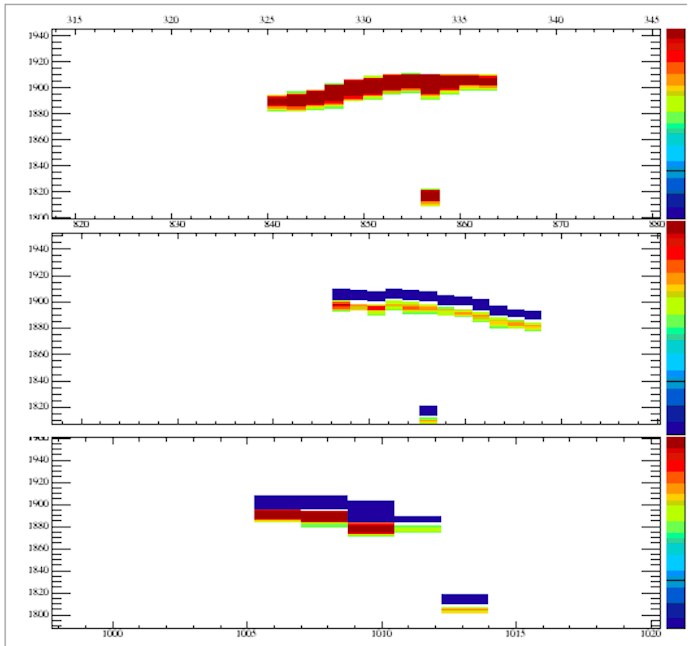
\includegraphics[width=0.6\textwidth]{snb-event-display.png}
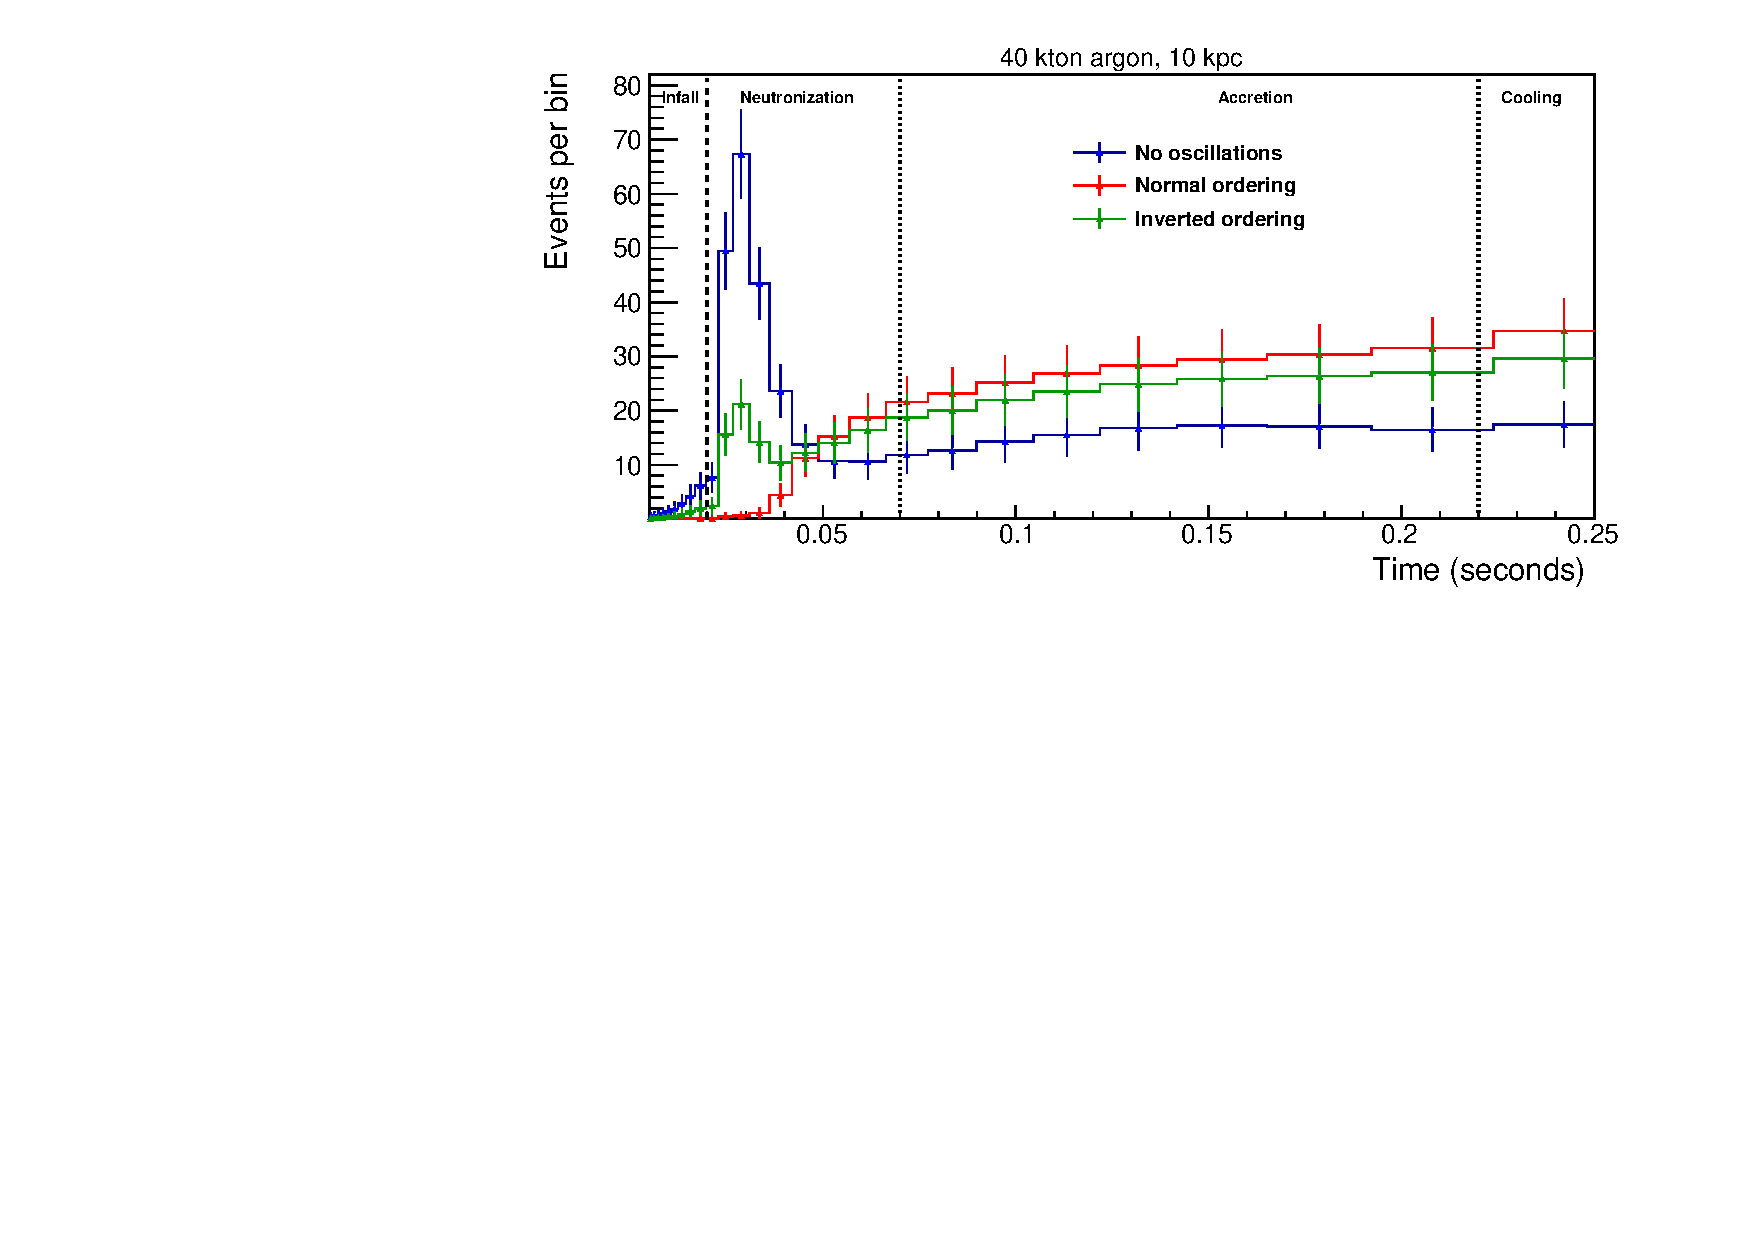
\includegraphics[width=0.8\textwidth]{early_time_argon.pdf}
\end{dunefigure}

Because no beam trigger is available for a supernova, efficient triggering and continuous data collection is critical for supernova neutrino burst physics. To fully capitalize on the physics opportunities, the DUNE far detector must provide event timing capability at the sub-millisecond level, must have spatial readout granularity sufficient to track electrons down to 5 MeV with good energy resolution, and must operate at noise levels and thresholds that allow detection and energy measurement for deexcitation gammas and nucleons at the MeV level.  The \lartpc technologies underlying the DUNE far detector conceptual designs is capable of meeting these requirements.

We note that information from DUNE will be highly complementary with neutrino burst information from other detectors, and furthermore multi-messenger astronomy information (from gravitational waves and a broad range of electromagnetic wavelengths) will combine to provide a full picture of a core-collapse event.


\subsection{The Core-Collapse Neutrino Signal}

\subsubsection{Core Collapse and Neutrino Production}

\subsection{Physics and Astrophysics Signatures}

\subsection{Low-Energy Neutrinos in LAr}

\subsubsection{Interaction Channels}

\subsection{Reconstruction of Low-Energy Neutrinos in DUNE}

\subsubsection{Low-Energy Event Reconstruction}

\subsubsection{Backgrounds}

\subsubsection{Predicted Event Rates}

\subsection{Physics Sensitivities and Detector Requirements}

\subsubsection{Triggering and DAQ}

This will be a summary of the relevant part of the TDR.

%%%%%%%%%%%%%%%%%%%%%%%%%%%%%%%%%%%%%%%%%%%%%%%%%%%%%%%%%%%%%%
\section{Solar neutrinos}
\label{sec:snb-lowe-solar}



\subsection{Expected Signal}

\subsection{Backgrounds}

\subsection{Sensitivities}

%%%%%%%%%%%%%%%%%%%%%%%%%%%%%%%%%%%%%%%%%%%%%%%%%%%%%%%%%%%%%%
\section{Supernova relic neutrinos}
\label{sec:snb-lowe-relic}

\subsection{Expected Signal}

\subsection{Backgrounds}

\subsection{Sensitivities}

